\section{Results}

\subsection{Nuclear Material Inventory}

\Cref{tab:sim_result1} lists \gls{EU} material inventory in 2050.
The materials continue to accumulate after 2050, but the
\gls{UNF} France receives before 2050 is most impactful for the
feasibility of the transition.


\begin{table}[h]
	\centering
%	\scalebox{0.86}{
		\begin{tabular}{ccc}
			\hline
			\textbf{Category } & \textbf{Value [MTHM]} & \textbf{Specifics}\\ \hline
			UOX Usage  & 158,794 &  \\ 
			MOX Usage  & 6,671  & \\ 
			\textbf{Used UOX Stored}  & \textbf{95,161}  & \gls{UNF} that is not reprocessed\\
			\textbf{Used UOX Stored (France)} & \textbf{9,979}  & \gls{UNF} that is not reprocessed \\
			Tails  & 979,463  & \\ 
			Natural U Used  & 1,141,916  & \\ \hline
		\end{tabular}
		\caption{Nuclear material inventory in the \gls{EU} in 2050 is summarized. 
				 The difference between total \gls{UOX} usage and \gls{UOX} stored is the amount
				 that has been reprocessed for \gls{MOX}. Only the stored \gls{UOX} is used for \gls{ASTRID} fuel production.}
		\label{tab:sim_result1}
\end {table}
\FloatBarrier


Figures \ref{fig:eu_tail} and \ref{fig:eu_snf} show the 
accumulation of tails and used fuel over time in the \gls{EU}.
Tails accumulate as a by-product of uranium enrichment. For every
ton of \gls{UOX} fuel, about nine times of tails is produced. 
Spent fuel is discharged from reactors every refueling period.
The entire core is discharged when the reactor decommissions.
A total of about $1,000,000 MTHM$ of tails and $100,000 MTHM$ of
\gls{UNF} accumulate in 2050.
Figure \ref{fig:eu_fuel} shows the amount of fuel used in \gls{EU}.


\begin{figure}[htbp!]
	\begin{center}
		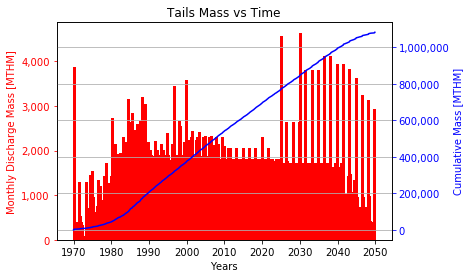
\includegraphics[scale=0.7]{./images/eu_future/tails.png}
	\end{center}
	\caption{This plot shows the timeseries of tails mass accumulation and discharge in the \gls{EU} nations.
			 Tails mass accumulation is fairly steady, with peaks occurring when
			 new reactors are deployed.}
	\label{fig:eu_tail}
\end{figure}

\begin{figure}[htbp!]
	\begin{center}
		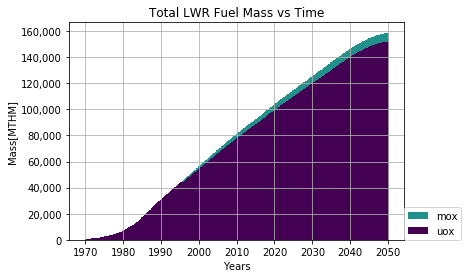
\includegraphics[scale=0.7]{./images/eu_future/total_fuel.png}
	\end{center}
	\caption{This plot shows the timeseries of total fuel usage in the \gls{EU} nations.}
	\label{fig:eu_fuel}
\end{figure}


\begin{figure}[htbp!]
	\begin{center}
			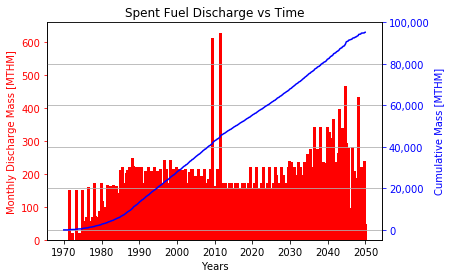
\includegraphics[scale=0.7]{./images/eu_future/snf_discharge.png}
	\end{center}
	\caption{This plot displays the timeseries of \gls{UNF} accumulation and discharge in the \gls{EU} nations.
			 The peaks are caused by decommissioning of reactors, where all the core is sent to the repository.}
	\label{fig:eu_snf}
\end{figure}
\FloatBarrier


\begin{table}[h]
	\centering
	\begin{tabular}{ccc}
		\hline
		\textbf{Isotope} & \textbf{Mass Fraction in Used Fuel [\%]} & \textbf{Quantity [t]} \\ \hline
		Pu238 & 0.0111 & 10.5628 \\ 
		Pu239 & 0.518 & 492.93 \\ 
		Pu240 & 0.232 & 220.7 \\ 
		Pu241 & 0.126 & 119.9 \\ 
		Pu242 & 0.0487 & 46.3 \\ \hline
		\textbf{Total} & \textbf{0.9358} & \textbf{890.5} \\ \hline
	\end{tabular}
	\caption{Plutonium From \gls{UNF} Inventory. This table assumes no decay
			 took place. The long half-life of the fissile Pu-239 (24,100 years)
			 weakens the impact of decay on the usability of \gls{UNF}.}
	\label{tab:pu}
\end{table}



\subsection{French \gls{SFR} Deployment}

Reprocessing \gls{UNF} collected from all EU nations can start approximately
180 \glspl{SFR}. Table \ref{tab:pu} lsits the isotope, mass fraction,
and quantity of plutonium that can be obtained from the 2050 \gls{UNF} inventory.
 With the \gls{SFR} breeding ratio above one, France can transition into
a fully \gls{SFR} fleet without extra construction of \glspl{LWR}. 

From Varaine et al. \cite{varaine_pre-conceptual_2012}, a French
ASTRID-type \gls{SFR} of capacity 600 \gls{MWe} needs $1.225$ tons of
plutonium a year, with an initial plutonium loading of $4.9$ tons. 
Thus, the number of \glspl{SFR} that can be loaded with the reprocessed
plutonium from \gls{UNF} can be estimated to $\frac{Pu \ from \ legacy \ \gls{UNF}}{4.9} \approx 181$ \glspl{SFR},
assuming abundant depleted uranium supply. 
 
Used \gls{MOX} from an ASTRID reactor is 23.95\% plutonium
in this simulation (see \cref{tab:comp}), whereas a fresh \gls{MOX} is 22\% plutonium.
The plutonium breeding ratio in this simulation is thus assumed to be
$\approx 1.08$.

\Cref{fig:fuel} shows \gls{MOX} loaded in the \glspl{SFR} per month.
The spikes are due to initial fuel demand for new deployment of \glspl{SFR}.
The initial loading of new \glspl{SFR} are done with the \gls{MOX} created
from legacy \gls{UNF}. Once the deployed \glspl{SFR} create enough amounts
 of extra plutonium, the legacy \gls{UNF} is no longer used. 

\begin{figure}[htbp!]
	\begin{center}
		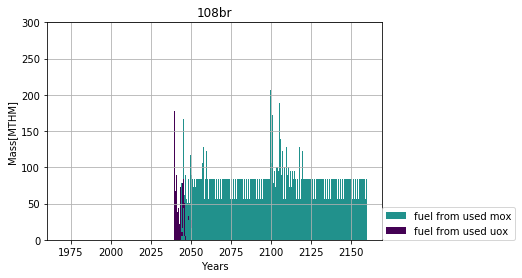
\includegraphics[scale=0.7]{./images/french-transition/where_fuel.png}
	\end{center}
	\caption{This plot shows the timeseries of fuel loaded into \glspl{SFR}.
			 The plot has peaks during a period of aggressive deployment of \glspl{SFR}
			 followed by an equilibrium at 150 \gls{MTHM}. The peaks reoccur with the
			 deployment of the second generation of \glspl{SFR}.}
	\label{fig:fuel}
\end{figure}
 \Cref{fig:pu_no_cum} shows the separated plutonium discharge
per month from the reprocessing plant. The plutonium outflux
does not precisely follow the fuel demand because \Cyclus agents have
material buffers that store commodity fuel for later usage. The reprocessed
plutonium from legacy \gls{UNF} is stored for the initial loading of \glspl{SFR}.
\Cref{tab:sfr_sim_result} lists metrics obtained from the second simulation.

\begin{figure}[htbp!]
	\begin{center}
		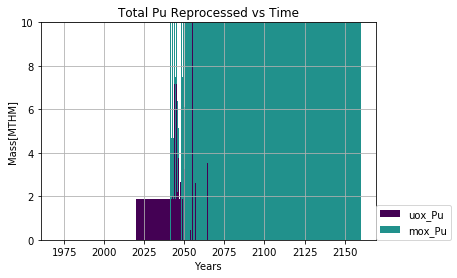
\includegraphics[scale=0.7]{./images/french-transition/pu.png}
	\end{center}
	\caption{This plot shows the separated plutonium discharge from the reprocessing plant.
			 The reprocessing demand for the first aggressive deployment of \glspl{SFR}
			 are lessened because the plutonium demand is met with plutonium separated from legacy \gls{UNF}.
			 The plutonium from reprocessing legacy fuel is a flat rectangle because the 
			 reprocessing throughput was set to 20 $\frac{tons}{month}$ to avoid reprocessing
			 all the legacy in one timestep. }
	\label{fig:pu_no_cum}
\end{figure}

\begin{table}[h]
	\centering
	\scalebox{0.86}{
		\begin{tabular}{ccc}
			\hline
			\textbf{Category} & \textbf{Unit} & \textbf{Value}  \\ \hline
			Total MOX used & MTHM & 63,820  \\ 
			\textbf{Average UOX Reprocessing} & MTHM/month & \textbf{118.92} \\
			\textbf{Average Total Reprocessing} & MTHM/month & \textbf{73.27} \\
			\textbf{Average Fuel Fabrication} & MTHM/month & \textbf{45.2} \\
			Total \glspl{SFR} Deployed & & 220 \\ 
			Total Plutonium Reprocessed & MTHM & 15,099 \\ 
			Total \gls{ASTRID} fuel from UOX Waste & MTHM & 2,923  \\ 
			Total \gls{ASTRID} fuel from MOX Waste & MTHM  & 60,535 \\ 
			Total Tails used & MTHM & 49,779 \\ 
			\textbf{Total legacy UNF reprocessed} & MTHM & \textbf{54,111} \\ 
			Total Reprocessed Uranium Stockpile & MTHM & 183,740 \\ 
			Total Raffinate & MTHM & 33,806 \\ \hline
		\end{tabular}}
		\caption {Listed are the metrics from the French transition to \gls{SFR} scenario.
				  The total legacy \gls{UNF} reprocessed is the amount of \gls{UNF} France would need
				  for a transition into a fully \gls{SFR} fleet. The tails used is around ninth
				  of the original tails inventory from the previous simulation.}
		\label{tab:sfr_sim_result}
\end {table}

Despite the large amount of initial plutonium that has to be reprocessed
prior to \gls{ASTRID} deployment, the 20 years of preparation of
\gls{ASTRID} fuel (2020-2040) allows a reasonable level of average
\gls{UOX} reprocessing capacity demand. \gls{UOX} reprocessing continues 
until 2057, when the \gls{ASTRID} spent fuel can supply the plutonium
for its own fuel.


